\documentclass[urlcolor=blue,dvipsnames]{beamer}

\usepackage[utf8]{inputenc}
\usepackage{fancybox,fancyvrb}
\usepackage{environ,xspace,empheq}
\usepackage{tikz}
\hypersetup{colorlinks,linkcolor=,urlcolor=cyan}

\beamertemplatenavigationsymbolsempty
\setbeamertemplate{footline}[frame number]
\usetheme{Pittsburgh}

\newcommand\enumnum[1]{{\renewcommand{\insertenumlabel}{#1}%
      \usebeamertemplate{enumerate item} \,}}

\newcommand{\grad}{\nabla}
\newcommand{\ih}{\boldsymbol{\hat{\textbf{\i}}}}
\newcommand{\jh}{\boldsymbol{\hat{\textbf{\j}}}}
\newcommand{\vF}{\boldsymbol{\vec{\textbf{F}}}}
\newcommand{\Matlab}{\textsc{Matlab}\xspace}
\newcommand{\Octave}{\textsc{Octave}\xspace}


\title{6.2 Series solutions about ordinary points}

\subtitle{a lesson for MATH F302 Differential Equations}

\author{Ed Bueler, Dept.~of Mathematics and Statistics, UAF}

\date{\tiny \today}


\begin{document}
\setbeamertemplate{itemize item}{$\bullet$}
\setbeamertemplate{itemize subitem}{$\circ$}
\renewcommand{\thefootnote}{{\color{green} \arabic{footnote}}}

\begin{frame}
\titlepage

\centerline{\tiny for textbook: \, D. Zill, \emph{A First Course in Differential Equations with Modeling Applications}, 11th ed.}
%\color{green!40!blue}
\end{frame}


\begin{frame}{series solutions of DEs}

\begin{itemize}
\item these slides are merely three gory exercises solving \emph{linear, homogeneous 2nd-order DEs} by power series methods
    \begin{itemize}
    \item two of which are DEs we could not previously solve
    \end{itemize}
\item recall the main idea of using series to solve DEs:

\medskip
\begin{enumerate}
\item substitute a series with unknown coefficients into the DE
\item find coefficients by matching on either side
\end{enumerate}

\medskip
\item see/do \S6.1 first \dots or these slides will not make sense!
\end{itemize}
\end{frame}


\begin{frame}{ordinary points}

\begin{itemize}
\item in \S6.2 we only use \emph{ordinary} base points for our series:

\medskip
\begin{quote}\normalfont
\emph{definition.}  Assume $a_2(x),a_1(x),a_0(x)$ are continuous, smooth, and well-behaved functions.\footnote{Precisely: \emph{analytic} functions.}  If $a_2(x_0)\ne 0$ then the point $x=x_0$ is an \emph{ordinary point} of the DE
    $$a_2(x) y'' + a_1(x) y' + a_0(x) y = 0$$
\end{quote}

\item we often write the same DE as
    $$y'' + P(x) y'' + Q(x) y = 0$$
where $P(x)=a_1(x)/a_2(x)$ and $Q(x)=a_0(x)/a_2(x)$
    \begin{itemize}
    \item $x=x_0$ is ordinary point if $P(x)$ and $Q(x)$ are analytic there
    \item \dots don't divide by zero
    \end{itemize}
\item a point which is not ordinary is \emph{singular} \dots see \S 6.3 \& 6.4

\bigskip
\end{itemize}
\end{frame}


\begin{frame}{summation notation realization}

\begin{itemize}
\item in these slides we do 2nd-order DEs only
\item so consider $y'$ and $y''$:
\small
\begin{align*}
\alert{y(x)} &= c_0 + c_1 x + c_2 x^2 + c_3 x^3 + \dots = \sum_{n=0}^\infty c_n x^n = \alert{\sum_{k=0}^\infty c_k x^k} \\
\alert{y'(x)} &= c_1 + 2 c_2 x + 3 c_3 x^2 + \dots = \sum_{n=0}^\infty n c_n x^{n-1} = \alert{\sum_{k=0}^\infty (k+1) c_{k+1} x^k} \\
\alert{y''(x)} &= 2 c_2 + 3 (2) c_3 x + \dots = \sum_{n=0}^\infty n (n-1) c_n x^{n-2} \\
       &= \alert{\sum_{k=0}^\infty (k+2)(k+1) c_{k+2} x^k}
\end{align*}
\item \alert{these forms} make summation notation an effective tool!
\end{itemize}
\end{frame}


\begin{frame}{an Airy equation}

\noindent \emph{exercise 1.}  find the general solution by series:
    $$y''+xy=0 \hspace{60mm}$$

\vspace{20mm}

\hfill \footnotesize $\displaystyle \boxed{\begin{matrix} 2\cdot 1\cdot c_2 = 0 \\
                                     3\cdot 2\cdot c_3 = -c_0 \\
                                     4\cdot 3\cdot c_4 = -c_1 \\
                                     5\cdot 4\cdot c_5 = -c_2 \\
                                     6\cdot 5\cdot c_6 = -c_3 \\
                                     7\cdot 6\cdot c_7 = -c_4 \\
                                      \vdots \\
                      \end{matrix}}$
\end{frame}


\begin{frame}{exercise 1, cont.}

\vspace{50mm}

\small
\begin{empheq}[box=\fbox]{align*}
  y_1(x) &= 1 - \frac{1}{3 \cdot 2} x^3 + \frac{1}{6 \cdot 5 \cdot 3 \cdot 2} x^6 - \frac{1}{9 \cdot 8 \cdot 6 \cdot 5 \cdot 3 \cdot 2} x^9 + \dots \\
  y_2(x) &= x - \frac{1}{4 \cdot 3} x^4 + \frac{1}{7 \cdot 6 \cdot 4 \cdot 3} x^7 - \frac{1}{10 \cdot 9 \cdot 7 \cdot 6 \cdot 4 \cdot 3} x^{10} + \dots
\end{empheq}

    $$y(x) = c_1 y_1(x) + c_2 y_2(x)$$
\end{frame}


\begin{frame}{exercise 1, cont.$^2$}

\begin{itemize}
\item what do these Airy\footnote{George Airy was an astronomer: \href{https://en.wikipedia.org/wiki/Airy_function}{\scriptsize \texttt{en.wikipedia.org/wiki/Airy\_function}}.} functions look like?
    \begin{itemize}
    \item I wrote a code to plot approximations to $y_1(x),y_2(x)$
    \item \dots by summing first twenty terms of the series
    \end{itemize}
\item Airy functions smoothly connect a kind of exponential growth (left side of figure) to sinusoid-ish stuff (right side)
\end{itemize}

\begin{center}
\begin{minipage}[t]{0.3\textwidth} \vspace{0mm} $y''+xy=0$\end{minipage}
\qquad\quad
\begin{minipage}[t]{0.55\textwidth} \vspace{-3mm} 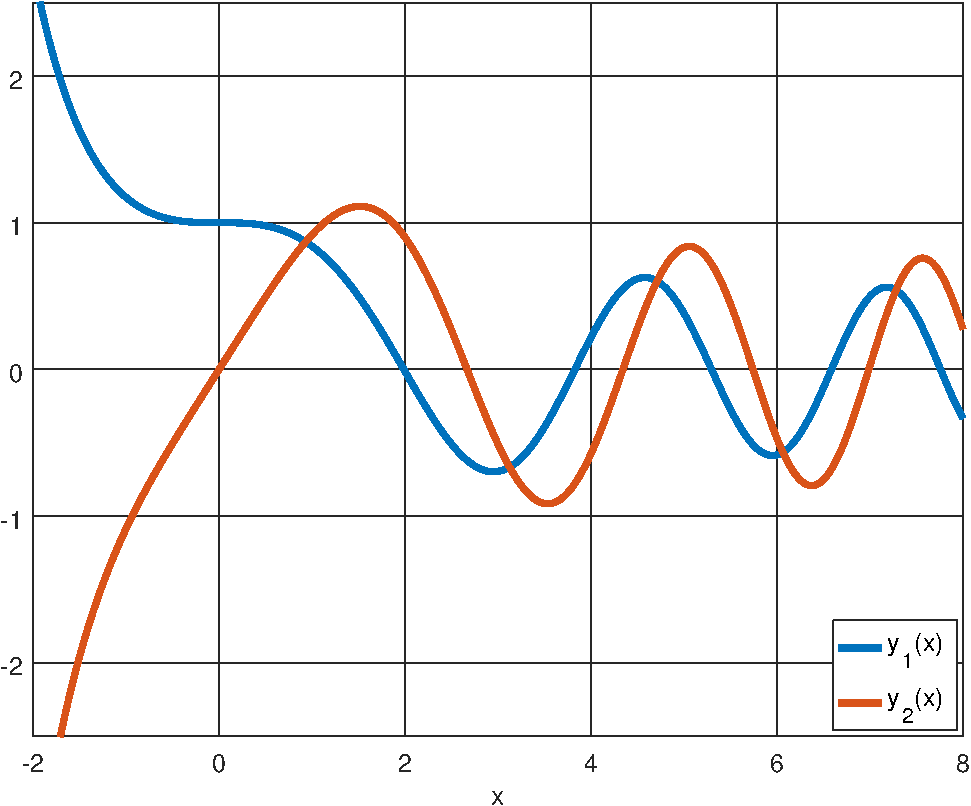
\includegraphics[width=\textwidth]{figs/airyplots} \end{minipage}
\end{center}
\end{frame}


\begin{frame}{problem easier than this will be on the quiz}

\noindent \emph{exercise 2.}  \qquad $y''+3y'-4y=0$, \quad $y(0)=1$, \, $y'(0)=1$

\begin{itemize}
\item[(a)] solve the IVP by any means you want
\end{itemize}

\vspace{50mm}
\end{frame}


\begin{frame}{exercise 2, cont.}

\begin{itemize}
\item[(b)] solve the IVP (\small $y''+3y'-4y=0$, $y(0)=1$, $y'(0)=1$\normalsize) by series
\end{itemize}

\vspace{45mm}

\hfill \footnotesize $\displaystyle \boxed{\begin{matrix} 2\cdot 1 c_2 + 3 \cdot 1 c_1 - 4 c_0 = 0 \\
                                     3\cdot 2 c_3 + 3 \cdot 2 c_2 - 4 c_1 = 0 \\
                                     4\cdot 3 c_4 + 3 \cdot 3 c_3 - 4 c_2 = 0 \\
                                     5\cdot 4 c_5 + 3 \cdot 4 c_4 - 4 c_3 = 0 \\
                                      \vdots \\
                      \end{matrix}}$
\end{frame}


\begin{frame}{exercise 2, cont.$^2$}

\vspace{60mm}

\footnotesize
\hfill $y(x) = 1 + x + \frac{1}{2} x^2 + \frac{1}{3\cdot 2} x^3 + \frac{1}{4\cdot 3\cdot 2} x^4 + \dots = e^x$
\end{frame}


\begin{frame}{get radius of convergence \emph{in advance!}}

\begin{itemize}
\item when you find a series solution you can then use the ratio test (etc.) to determine radius of convergence $R$
\item \dots but this is unwise!
\item Theorem 6.2.1 on page 245 tells us that

\medskip
\begin{quote}
\normalfont \alert{a minimum for $R$ is the distance, \emph{in the complex plane}, from the basepoint $x=x_0$ to the nearest singular point}
\end{quote}

    \begin{itemize}
    \item $a_2(x) y''+ a_1(x) y' + a_0(x) y=0$: anywhere $a_2(x)=0$ is a singular point
    \item $y''+P(x)y'+Q(x)y=0$: anywhere $P(x)$ or $Q(x)$ is not analytic is a singular point
    \end{itemize}
\end{itemize}
\end{frame}


\begin{frame}{like \#2 in \S 6.2}

\noindent \emph{exercise 3.}  {\color{Blue} (a)} without actually solving the DE, find the minimum radius of convergence of the power series solutions about $x=0$:
  $$(x^2+1) y'' - 6 y = 0$$

\vspace{15mm}
\begin{itemize}
\item[(b)] same, but about $x=2$
\end{itemize}

\hfill 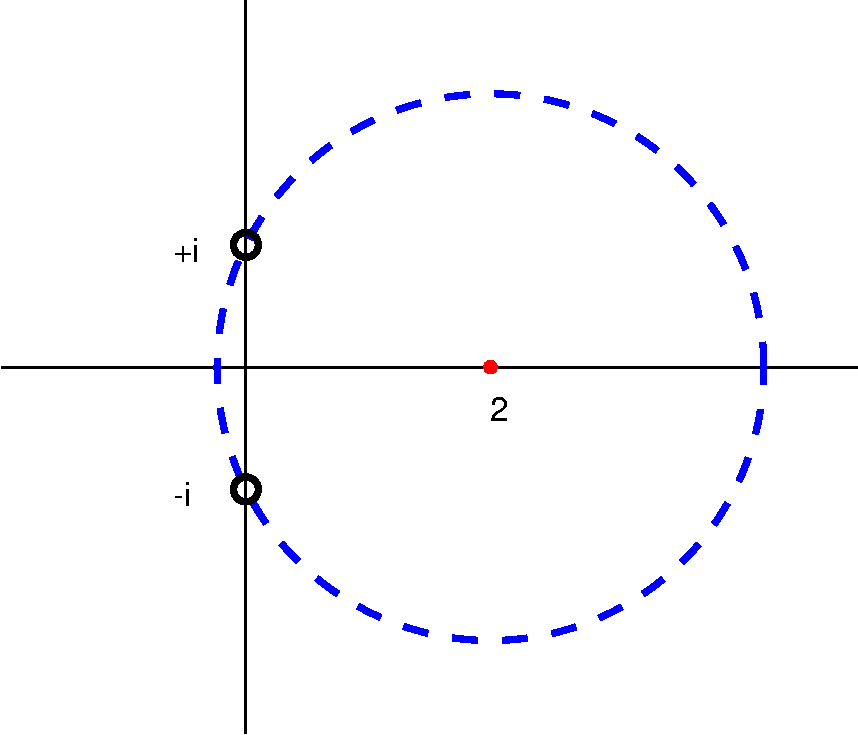
\includegraphics[width=0.35\textwidth]{figs/minradius}
\end{frame}


\begin{frame}{exercise 3, cont.}

\begin{itemize}
\item[(c)] find two series solutions about $x=0$: \small\quad $(x^2+1) y'' - 6 y = 0$
\end{itemize}

\vspace{40mm}

\hfill \footnotesize $\displaystyle \boxed{\begin{matrix} 2\cdot 1 c_2 - 6 c_0 = 0 \\
                                     3\cdot 2 c_3 - 6 c_1 = 0 \\
                                     2\cdot 1 c_2 + 4\cdot 3 c_4 - 6 c_2 = 0 \\
                                     3\cdot 2 c_3 + 5\cdot 4 c_5 - 6 c_3 = 0 \\
                                     4\cdot 3 c_4 + 6\cdot 5 c_6 - 6 c_4 = 0 \\
                                      \vdots \\
                      \end{matrix}}$
\end{frame}


\begin{frame}{exercise 3, cont.$^2$}

\vspace{45mm}

\footnotesize
\begin{empheq}[box=\fbox]{align*}
  y_1(x) &= 1 + \frac{6}{2 \cdot 1} x^2 + \frac{(6-2\cdot 1)(6)}{4!} x^4 + \frac{(6-4\cdot 3)(6-2\cdot 1)(6)}{6!} x^6 + \dots \\
  y_2(x) &= x + \frac{6}{3 \cdot 2} x^3 + \frac{(6-3\cdot 2)(6)}{5!} x^5 + \frac{(6-5\cdot 4)(6-3\cdot 2)(6)}{7!} x^7 + \dots
\end{empheq}

    $$y(x) = c_1 y_1(x) + c_2 y_2(x)$$
\end{frame}


\begin{frame}{was this progress?}

\begin{itemize}
\item yes, we can solve more DEs than we could before
    \begin{itemize}
    \item \alert{we have escaped from \S4.3 constant-coefficient DEs}
    \end{itemize}
\item \emph{but}, to understand what you get, you must spend quality time with series-defined functions $y_1(x)=\dots$ and $y_2(x)=\dots$
\item this is worthwhile in some famous cases:
\begin{align*}
y''-xy &= 0 &\implies &&\text{Airy functions} \\
x^2 y'' + xy' + (x^2-\nu^2) y &= 0 &\implies &&\text{Bessel functions} \\
(1-x^2) y'' - xy' + \alpha^2 y &= 0 &\implies &&\text{Chebyshev functions} \\
 &&\vdots &&
\end{align*}
\item i.e.~\emph{special functions}
\end{itemize}
\end{frame}


\begin{frame}{historical comment}

\begin{itemize}
\item from about 1800 to 1950, finding new series solutions to DEs was the kind of thing that mathematicians and physicists did for a living
    \begin{itemize}
    \item you could get your name on some new special functions!
    \item e.g.~Bessel, Legendre, Airy, Hermite, \dots \S 6.4
    \end{itemize}
\item with powerful computers and software (since 1980?) one may/should automate the creation of series solutions
    \begin{itemize}
    \item naming new special functions is no longer a thing
    \item I'm describing the invention of Mathematica
    \item \dots and then \href{https://www.wolframalpha.com/}{Wolfram Alpha}
    \item the quality of approximations \emph{is} still a thing
    \end{itemize}
\end{itemize}
\end{frame}


\begin{frame}{expectations}

\begin{itemize}
\item just watching this video is \emph{not} enough!
     \begin{itemize}
     \item see ``found online'' videos and stuff at

     \centerline{\href{https://bueler.github.io/math302/week9.html}{\tt \color{cyan} bueler.github.io/math302/week9.html}}
     \item \emph{read} section 6.2 in the textbook
     \item \emph{do} the WebAssign exercises for section 6.2
     \end{itemize}
\item we will skip \S 6.3 \& 6.4
\end{itemize}
\end{frame}

\end{document}

